\section{Architecture}

Modern computer science emphasize parallelism as a highly important property in
order to achieve speed on multicore processors. As the size of the log files
which PET has to parse can easily be 10s of gigabytes large, PET has to be
designed with performance in mind. This means that PET must be lightweight and
parallel in order to be fast, while it must maintain correctness and be easy to
use.

Due to memory constraints on commonly available computers, it is not feasible to
read the entire log file into memory and then start parsing. It would also make
the reading step a serial part of the program, which hinders parallelism. It
will also be a bad idea to read one line, parse it, weight it and apply it to
the grand total, as it would be an entirely serial process.

\subsection{Overview}

\begin{figure}[ht]
    \includegraphics[width=0.9\textwidth]{figs/pet-pipeline-gv.pdf}
    \caption{How PET works}
    \label{fig:pipeline}
\end{figure}

In order to maintain good speed while still keeping the PET source code
readable, we have looked at different ways of chewing through large data sets.
The final implementation of PET follows a scheme borrowing ideas from the
producer-consumer patterb as explained by Gamma et. al. in \cite{designpatterns}
and the MapReduce algorithm \cite{dean2008mapreduce}. As depicted in
\autoref{fig:pipeline}, this scheme makes it rather easy to let a producer read
the lines from the log file into ring buffers (produce) and let multiple
consumers pick from each their ring buffer (consume). Each consumer parses the log
lines they pick, and apply the weight of each read event to each their result
vector (map). When all lines are read and parsed, the results vectors are
merged, and idle-task power and static power consumption is added (reduce). This
combination of algorithms allows PET to take advantage of as many cores as
possible, limted only by how fast the producer can read the log files. Finally,
a human readable output is produces, either as a gnuplot line graph or as
formatted or plain text output.


\subsection{Argument Parsing and Program Options}

As any other non-trivial programs, PET has to adapt to input options given from
the command line or from a settings-file. PET makes extensive use of the
\texttt{Boost}-library \cite{boostwebpage} and utilize
\texttt{Boost::Program\_options} for parsing the command line. Making use of
\texttt{Boost} for common tasks all over the program made the development cycle
less cumbersome and more rapid. \texttt{Boost::Program\_options} allows easy
extraction of program options, both with long (\texttt{\textemdash \textemdash
option=\emph{value}}) and short (\texttt{\textemdash o~\emph{value}})option
style.


\subsection{Reading Trace Logs}

When arguments are parsed and a trace log has been specified, either by path or
as \texttt{stdin}, a single thread is kicked off reading each line of the log
file into a C++ string container. The string container is then inserted into one
of many circular buffers. The circular buffers are implemented with
\texttt{boost::lockfree::spsc\_queue}, a lock free single producer, single
consumer queue. The property of beeing lock free is explained by Tim Blechmann
and the boost-community in \cite{boostlockfree} as follows: "data structures are
\emph{lock-free}, if some concurrent operations are guaranteed to be finished in a
finite number of steps. While it is in theory possible that some operations
never make any progress, it is very unlikely to happen in practical
applications". In PET, this queue has a fixed size of 8192, but dynamic size is
also available in the library implementation.

Which buffer the string is inserted into is determined by a simple circular
algorithm; the next ring buffer is selected when current one is full. When the
buffers are small enough to be filled fast enough to let all workers do work,
this method creates a lot less locking than using a single ring buffer shared by
all worker threads. The number of threads and the size of the ring buffers are
tightly coupled with how fast the host computer is able to feed PET with the log
files.

It is our experience that reading the log file is not the bottle neck, and it is
easy to feed at least 8 cores when the log file is hosted on a reasonable fast
drive. A simple benchmarking done with PET running on a system consisting of an
Intel Core i7 4820, 32GB DDR3 SDRAM and keeping the log files on a fake-RAID
Level-0 consisting of two Western Digital Caviar Black 750GB disks shows this.
PET running with 8 threads on this particular system is consuming the log files
with a rate of 133MB/s regardless of where the log files resides in RAM or on
disk. The benchmark used a log file of 5458MB and was run in 40.871 seconds.

\subsection{String to Event Mapping and Power Accumulation}

As the producer fills the ring buffers for each of the workers, the workers pick
strings from their pool. The strings are pop'ed from the ring buffer, thus making space
for new elements right away. Each string is parsed by the TraceLine class, which looks
for 

\subsection{Data Reduction}

\subsection{Output Production and Annotations}

\subsection{Unit Tests}


\subsection{Details}

PET is no huge nor advanced program, but it embeds features ranging from string
parsing functionality to thread pooling to number crunching. As seen in the call graph
in \autoref{fig:callgraph} PET starts out as any other ordinary program in it's main
function. PET is initialized and parses 


PET is a tool which main task will be to 

When designing a tool for parsing large input files and applying flexible configuration alternatives,
there are quite a few aspects that needs to be considered. Through this section the design choises
briefly explained in \autoref{sec:whatispet} will be further explained and more deeply understood.

PET has to be designed for good performance.


\begin{figure}
%    \includesvg[clean,eps,pretex=\relscale{0.25},width=\textwidth]{figs/maincallgraph}
    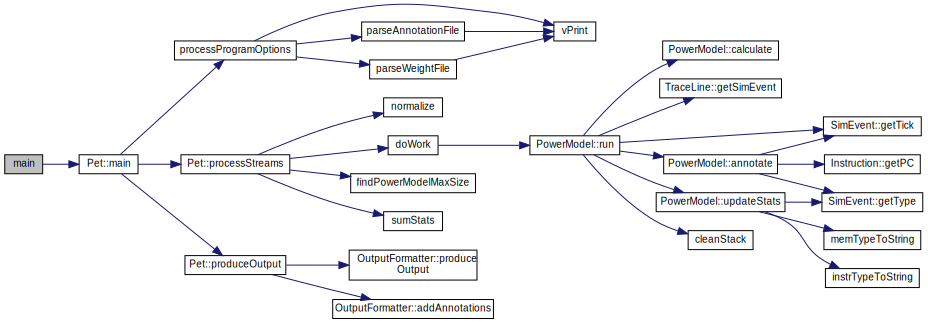
\includegraphics[width=\textwidth]{figs/maincallgraph.pdf}
    \caption{Call graph}
    \label{fig:callgraph}
\end{figure}

put UML-figures here
trådpool
concurency
arbeidsdeling
ringbuffer, statisk vs. ikke statis størrelse




